\documentclass[12pt]{article}

\usepackage{geometry,calc}
\usepackage{amsmath,amssymb,hyperref}

\def\quiztitle{Graded Problem 7}
\def\quizsubtitle{Math 4B,\qquad Spring 2017,\qquad Dr. Paul}
\pagestyle{empty}

\geometry{body={6.5in, 9in}, left=1in, top=1in}
\input{../../AxesFunction.tex}

\newcommand{\be}{\begin{enumerate}}
\newcommand{\ee}{\end{enumerate}}

\everymath{\displaystyle}

\begin{document}

%\hfill Student Name: \rule{2in}{.1pt}\\

%\hfill Section Time (e.g. 8am): \rule{2in}{.1pt}\\

\begin{center}
{\Huge \quiztitle}
\vskip.1in
{\large \quizsubtitle}
\end{center}

\begin{enumerate}

 \item A city's water system is set up as shown.
  
  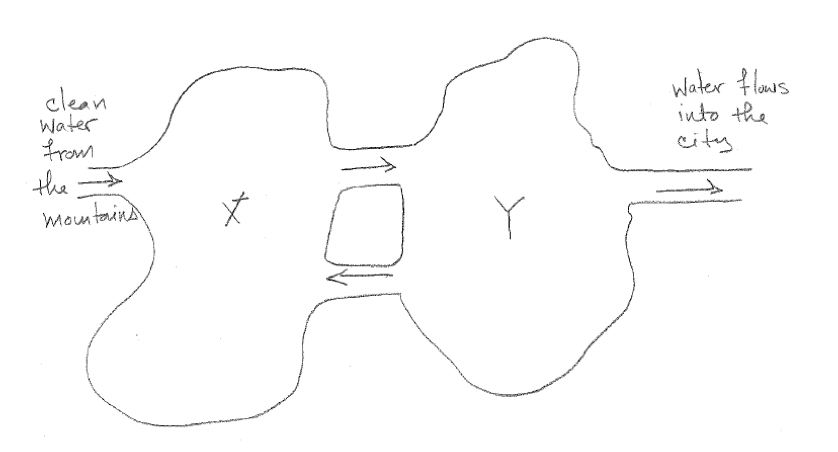
\includegraphics[scale=.5]{watersystem}
  
  Each of the two reservoirs holds 100 million gallons of water. Water flows into reservoir X from the mountains at a rate of 600,000 gallons, and out from reservoir Y to the city at the same rate. Water also circulates between the reservoirs: flowing from X to Y at a rate of 800,000 gallons per hour and from Y to X at a rate of 200,000 gallons per hour. Vector, the villian from \emph{Despicable Me}, dumped 1,500 lb sodium hypochlorite into reservoir X.
  
  \be
   \item Find a system of differential equations which models the amounts of sodium hypochlorite in each reservoir as functions $x(t)$ and $y(t)$ of time.
   
   \item If $u(t)=2x(t)+y(t)$, what is $u'(t)$ in terms of $u(t)$? Find the function $u(t)$.
   
   \item If $v(t)=2x(t)-y(t)$, what is $v'(t)$ in terms of $v(t)$? Find the function $v(t)$.
   
   \item Using the functions $u(t)$ and $v(t)$ above, find the functions $x(t)$ and $y(t)$. 
   
   \item Write a few sentences explaining how the process you used here relates to our eigenvector/alue method from class.
   
   \item How long does it take for the concentration in Y to get down to 3 lb/million gallons?
   
 \ee

\end{enumerate}



\end{document}